\begin{figure}[H]
\centering
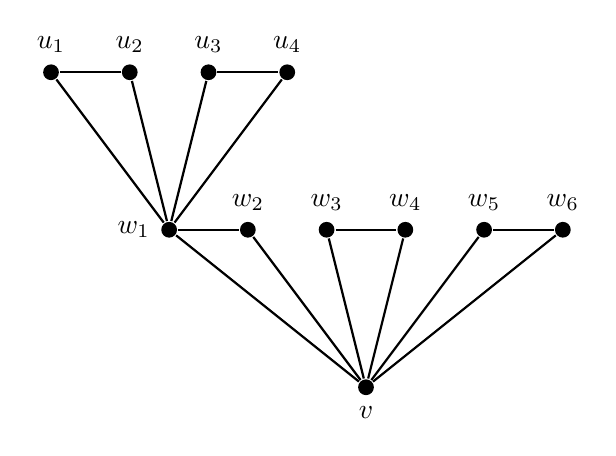
\begin{tikzpicture}[
       thick,
       acteur/.style={
         circle,
         fill=black,
         thick,
         inner sep=2pt,
         minimum size=0.2cm
       }
     ]

       \node (v) at (-3.5,0) [acteur,label=below:$v$]{};
       \node (w1) at (-6,2) [acteur,label=left:$w_1$]{}; 
       \node (w2) at (-5,2) [acteur,label=above:$w_2$]{}; 
       \node (w3) at (-4,2) [acteur,label=above:$w_3$]{};
       \node (w4) at (-3,2) [acteur,label=above:$w_4$]{};
       \node (w5) at (-2,2) [acteur,label=above:$w_5$]{};
       \node (w6) at (-1,2) [acteur,label=above:$w_6$]{};
       \node (u1) at (-7.5,4) [acteur,label=above:$u_1$]{};
  	   \node (u2) at (-6.5,4) [acteur,label=above:$u_2$]{};
  	   \node (u3) at (-5.5,4) [acteur,label=above:$u_3$]{};
  	   \node (u4) at (-4.5,4) [acteur,label=above:$u_4$]{};
  	   
       \draw (v) -- (w1);
       \draw (v) -- (w2);
       \draw (v) -- (w3);
       \draw (v) -- (w4);
       \draw (v) -- (w5);
       \draw (v) -- (w6);
       
       \draw (w1) -- (w2);
       \draw (w3) -- (w4);
       \draw (w5) -- (w6);
       
       \draw (w1) -- (u1);
       \draw (w1) -- (u2);
       \draw (w1) -- (u3);
       \draw (w1) -- (u4);
       
       \draw (u1) -- (u2);
       \draw (u3) -- (u4);
       

\end{tikzpicture}
  \caption{The case $f=0$}
  \label{figure9:Figure 9}
\end{figure}
